\subsection{Operating System Interaction and Management}
The operating system communicates with SSDs through storage drivers and the block I/O subsystem while 
relying on the SSD controller for flash memory management \cite{gfg_disk_mgmt}.

\subsubsection{File System Creation}
The operating system creates logical file systems such as NTFS, ext4, or APFS, allowing applications 
to organize and access stored data efficiently \cite{gfg_disk_mgmt}.

\subsubsection{Partitioning}
Similar to HDDs, SSDs can be divided into multiple partitions, enabling separate operating systems,
recovery partitions, or user data storage \cite{gfg_disk_mgmt}.

\subsubsection{I/O Scheduling}
Because SSDs have negligible seek time, traditional HDD scheduling algorithms provide little benefit. 
Modern operating systems therefore use simplified scheduling strategies that prioritize fairness and 
efficient request handling rather than minimizing head movement \cite{gfg_disk_mgmt}.

\subsubsection{TRIM Command}
The operating system periodically issues the TRIM command to notify the SSD which data blocks are 
no longer in use. This allows the SSD controller to erase unused blocks in advance, improving future 
write performance and reducing unnecessary wear \cite{openai2026nvmearchitecture}.

\subsubsection{Wear Leveling and Garbage Collection}
The SSD controller automatically distributes write operations across memory cells (wear leveling) 
and consolidates partially used blocks (garbage collection). These techniques increase storage 
lifespan and maintain consistent performance \cite{openai2026nvmearchitecture}.


\begin{figure}[H]
    \centering
    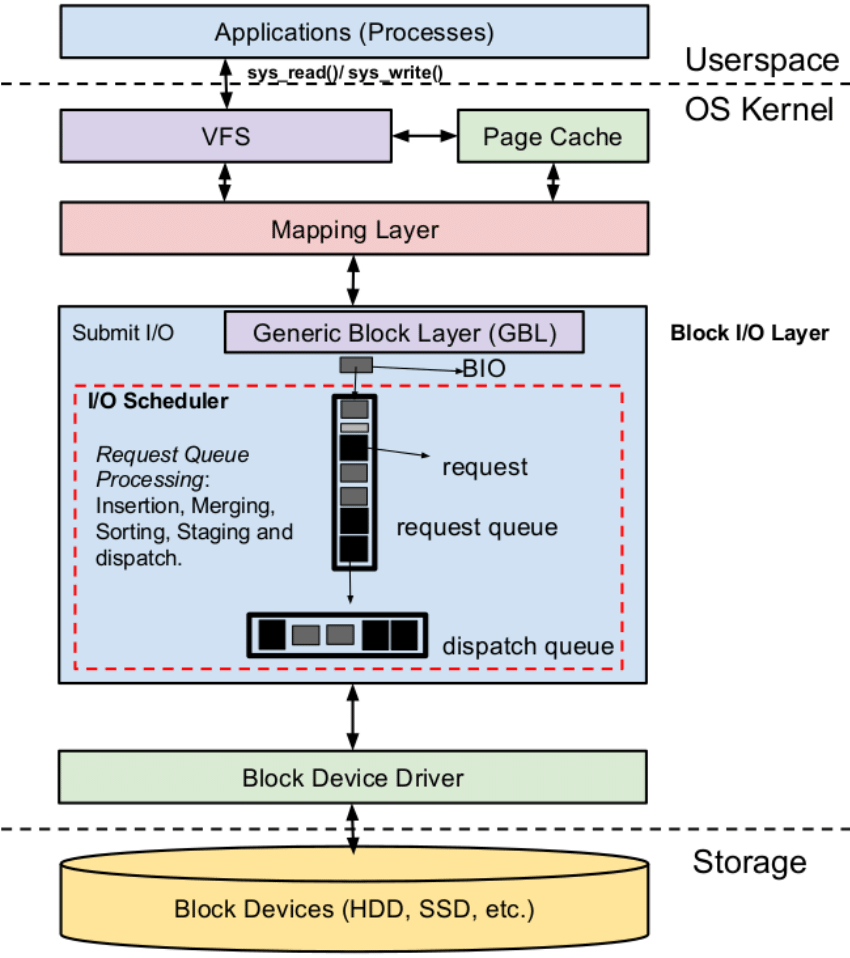
\includegraphics[width=0.5\linewidth]{ssd-os_interaction.png}
    \caption{OS Interaction with SSD}
    \label{fig: os_interaction_with_sata_ssd}
    
\end{figure}


